\entry{Semana del 11/07/2025}
\section{Lunes 07/07/2025.}

\subsection*{Notas del día.}
\begin{itemize}
	\item . Sigo con el mismo vaso con agua destilada y PhotFlo del viernes pasado. 
	\item Oscilaciones: 51.329 kHz, 51.359 kHz, 51.389 kHz parece ser cada 30 Hz. 
	
	\item A partir de ahora voy a usar el random\_interval para sacar las oscilaciones molestas, variando aleatoriamente un poco el tamaño de la ventana usada y que no sea siempre 8192. 
	\item Apretar el stand hace que se mueva el sensor tal que la fase salta 0.003 rad, por ahí eso está molestando en las calibraciones, que va shifteando el peso lentamente, pero igual esperaría que las curvas coincidan. 
	\item Cuando tornillo está completamente levantado salta menos, tipo 0.0015 rad. 
	
	\item Voy a hacer de abajo para arriba y viceversa y después de nuevo para arriba. Tornillo en 10 con 51.406 kHz.  
	\item Las curvas no se pegan. Hay en el transitorio para cada punto oscilaciones de 100 Hz, ¿serán las mismas que aparecían en el espectro?.
	
	\item Cuando lo mojo después tiene tendencia a irse para arriba y cuando lo seco después tiende tendencia irse para abajo. 
	
	\item Podemos probar con aceite de silicona o glicerina para ver si se pega más al alambre deberían separase más. 
	
	\item Voy a probar con el agua con PhotFlo pero tomando 0.4 s en vez de 0.1 por si el estacionario hace algo raro. En realidad, tardan según el timepo real unos 10 segundos en adaptarse. 
	
	\item Canal 1 referencia, canal 2 la misma referencia. En 124.711 kHz da mucho ruido. 
	\item No hacer el delay de medio punto efectivamente agrega una fase de $2\pi$ * $f$ * $\Delta$ $t$ con $\Delta t = 1\mu$ s. 
	
	\item Mover el stand del sensor da saltos también, por ahí la mesa está inclinada o algo así. Usar shaker o paralante. 
	\item Poner motor del wave driver con paleta o agarrador de vaso y mover eso con el motor vertical ya sea mirando para arriba y el vaso apoyado encima o mirando abajo y vaso tipo canastita. 
	\item Usar algo o el mismo diseño del sujetador del toriode pero con un diámetro menor donde entre el vaso y eventualmente trabe. 
	
	\item Hay drift con el sensor sin sumergir. 
	\item Tocar la punta del sensor da saltos de fase más altos que tocar otras partes del alambre, revisar si está bien aislado de alguna forma.  
\end{itemize}

\subsection*{Subir y bajar y volver a subir.} 
Seguimos con las pruebas para tratar de entender qué es lo que puede estar generando que las ramas no se peguen. Ahora agregué una vuelta más a la calibración y empecé desde abajo.

\begin{figure}[!ht]
	\begin{minipage}[c]{0.325\textwidth}
		\begin{subfigure}{\textwidth}
			\centering
			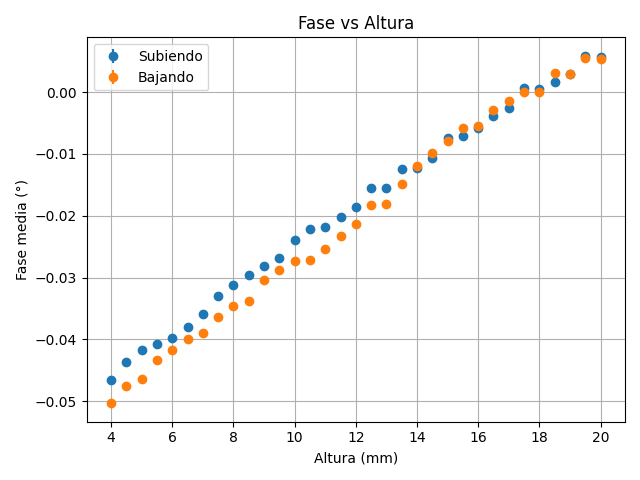
\includegraphics[width=0.98\textwidth]{Figures/07_07_2025/Subiendo_bajando.png}
		\end{subfigure}
	\end{minipage}\begin{minipage}[c]{0.3249\textwidth}
		\begin{subfigure}{\textwidth}
			\centering
			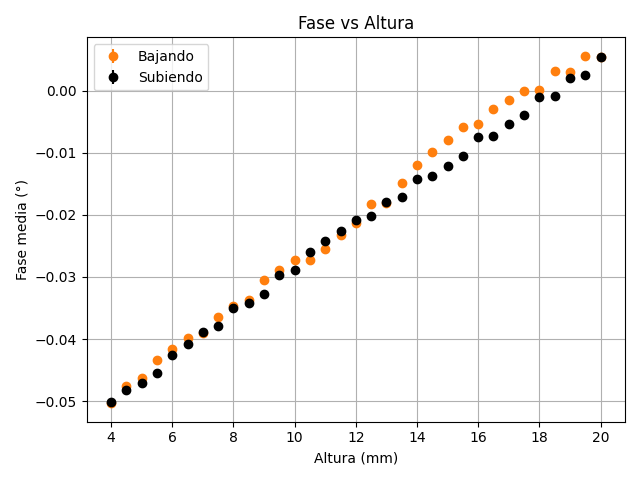
\includegraphics[width=0.98\textwidth]{Figures/07_07_2025/Bajando_subiendo.png}
		\end{subfigure}
	\end{minipage}\begin{minipage}[c]{0.3249\textwidth} %&} 
		\begin{subfigure}{\textwidth}
			\centering
			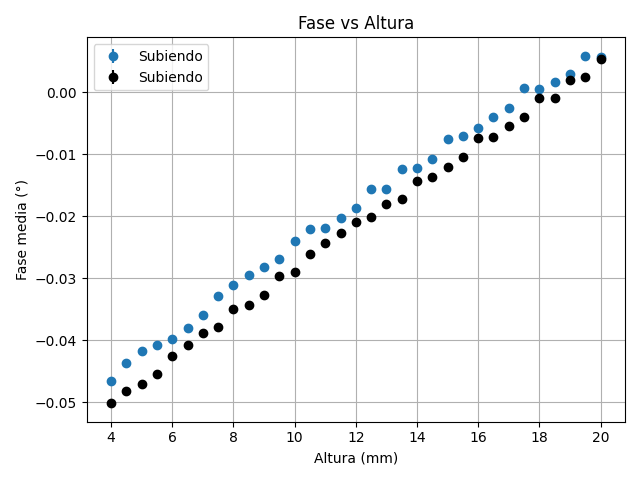
\includegraphics[width=0.98\textwidth]{Figures/07_07_2025/Subiendo_Subiendo.png}
		\end{subfigure}
	\end{minipage}
	\caption{Calibración para el mismo setup que lo último pero ahora en un ciclo de primero subir, después bajar y después volver a subir. } % Hola 
	\label{fig:calibración_otra_dirección}
\end{figure} 

Podemos ver para empezar que la dirección del movimiento importa, según si empezamos arriba o abajo se abren en uno u otro lugar. Además las dos subidas tienen la misma pendiente pero con un offset luego de la bajada intermedia. 




\section{Viernes 11/07/2025.} 
\subsection*{Notas del día:}
\begin{itemize}
	\item Voy a probar obtener la amplitud y fase del RLC n función de la frecuencia como su respuesta a una cuadrada. 
	\item Parece que describe bien la curva de resonancia pero muy llena densamente como para extraer directo de ahí la frecuencia de amplitud máxima. Además está montada sobre el 1/x de la cuadrada. 
	
	\item Con ruido blanco y Welch parece que funciona mejor pero hasta cierto punto.  
	
	\item Al variar el sensor va a cambiar la altura respecto del fondo, no sé que tanto cambiará eso la respuesta, por ahí en Shallow waters es más relevante. 
	
\end{itemize}
\subsection*{Ideas.}
La idea sería poder sistematizar la calibración para poder repetirla en distintos líquidos (por ejemplo aceite siliconado o glicerina) con distintas viscosidades y determinar finalmente si lo que separa las ramas es algún efecto de wetting y tensión superficial u otra cosa. Para esto tenemos la idea hace rato de usar ya sea el shaker o el parlante pero siento que no llegan a los 2 cm de amplitud que podemos variar con el tornillo micrométrico como para que vaya a ser comparable. Lo otro que se me ocurrió hoy sería usar el wavedriver puesto verticalmente en la cuba con una paleta que sostenga un recipiente con agua destilada u otro líquido, y este sí llegaría a moverse fácilmente 2 centímetros. % , 

\subsection*{Determinación rápida de la resonancia.} 
Otra cosa que me puse a probar mientras terminábamos de cerrar la idea de la calibración fue una forma más rápida para obtener la frecuencia de resonancia de un sistema (amplitud máxima y fase 0°), ya que hacer el barrido en frecuencias manualmente lleva bastante tiempo en comparación a otras cosas y el graficador en tiempo real tiene artefactos que no permiten que confíe en eso al 100 \%. 

Probé varias cosas. En un primer lugar quería hacer algo parecido a la práctica de Laboratorio 2 en ultrsonido donde pegamos una patada con el parlante (aunque no es exactamente lo mismo que esto). Para esto usé una cuadrada de frecuencia baja (en Fourier va como ~$1/f$ la amplitud con picos en $nf_0$). Después tomo una muestra del canal 2 sobre la resistencia y le hago la FFT. 

\begin{figure}[th!]
	\centering
	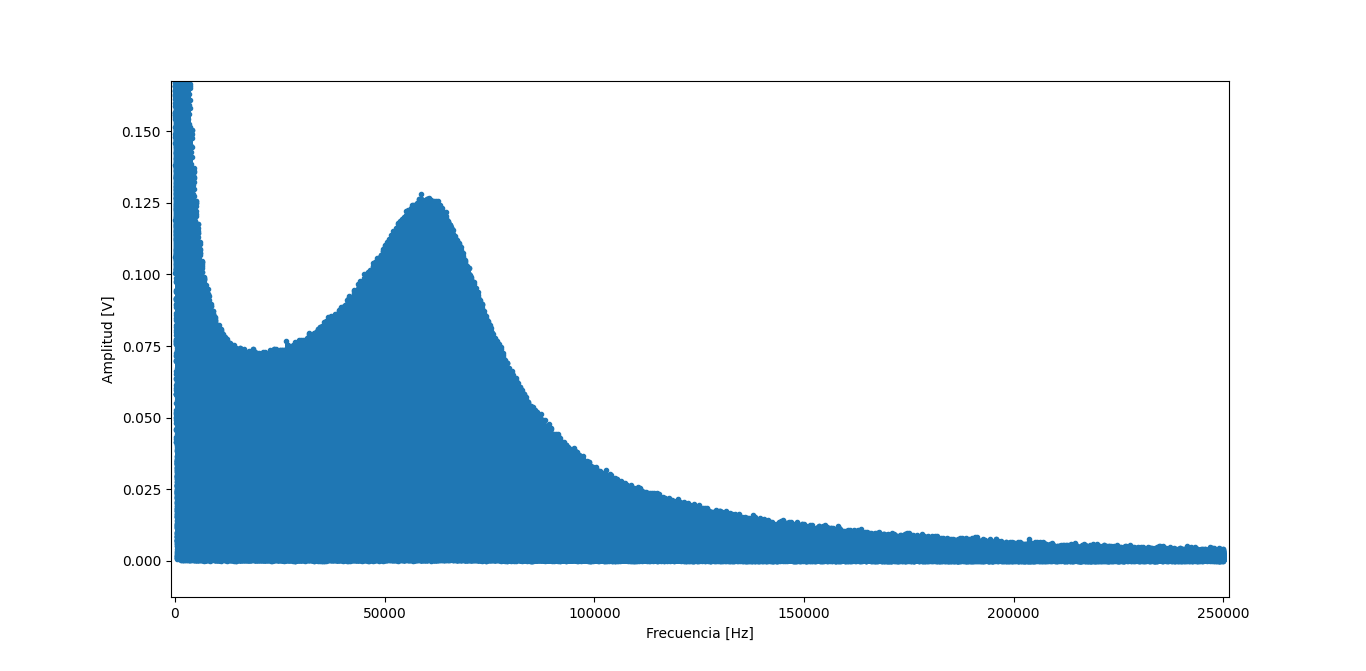
\includegraphics[width=0.87\linewidth]{Figures/07_07_2025/Respuesta_cuadrada_10Hz}
	\caption{Respuesta en frecuencia a una cuadrada de 10 Hz para un circuito RLC serie midiendo sobre la resistencia el voltaje con la DAQ.}
	\label{fig:respuestacuadrada10hz}
\end{figure}

Efectivamente vemos que se ve el pico en una resonancia pero está montado sobre el $1/f$. Además esta disminución en frecuencia hace que para frecuencias altas (donde está la de resonancia que nos interesa) tengamos menor resolución, y habría que tomar la envolvente de alguna forma de todos los picos. Probé para cuadradas de otras frecuencias, más bajas (1 Hz) y más altas (1 kHz, 10 kHz) pero el comportamiento es el mismo.

\vspace{2em} 
Después probé usar ruido blanco, que debería tener amplitud constante en frecuencia (aunque el que sale del generador es constante tiene ruido la amplitud ya que se genera aleatoriamente).  

\begin{figure}[th!]
	\centering
	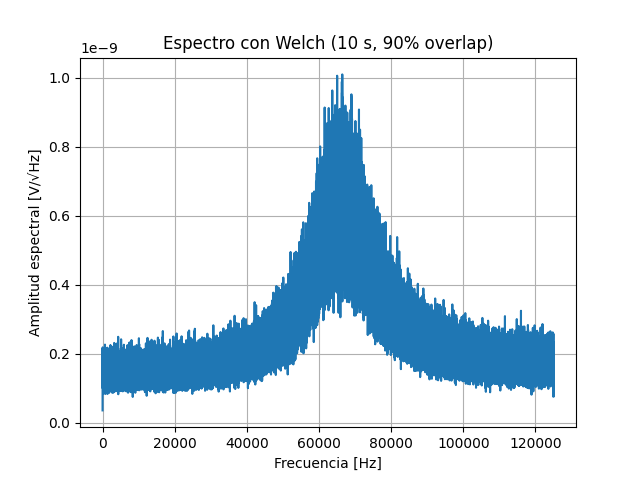
\includegraphics[width=0.87\linewidth]{Figures/07_07_2025/Ruido_blanco_Welch}
	\caption{Respuesta en frecuencias al ruido blanco del generador de un RLC serie midiendo sobre la resistencia con la DAQ y aplicando Welch.}
	\label{fig:ruidoblancowelch}
\end{figure} 

Para poder distinguir el pico entre el ruido usé Welch directamente sobre los datos y efectivamente aparece el pico. 

